\chapter{Tagsets with Style}
\index{Styles}
The fundamentals of tagsets have been covered, now it is time
do something with them. 
This chapter will cover examples that specifically leverage
ODS styles to accomplish their tasks.

\section{A Problem with Table Rules}
\index{Table!rules}
\index{Table!borders}
\index{Table!style}
The tables that ods generates are fairly basic.  Most people 
probably never take a second look at their style.  Sometimes
there are special needs for the way a table is done.  Most
often that has to do with the rules, or lines, that outline
the table.  Previous to SAS 9.1 ODS styles provided four 
attributes to control these, frame, rules, bordercolor 
and borderwidth. If those four don't help then 
things are going to be more difficult.

Table \ref{table_attribute rules} shows the style attributes that control
table rules.  The extended attributes\footnote{Available experimentally in SAS 9.1} 
are shown in table \ref{table_attribute rules2}.

\begin{table}\caption{Table border controls}
\label{table_attribute rules}
\begin{tabular}{l|l|l} \\ \hline
frame & \multicolumn{2}{|l}{Controls the frame around the table}\\
      & Void & No frame. \\
      & Above & Frame on top \\
      & Below & Frame on bottom \\ 
      & HSides & Frame on the Horzontal sides \\ 
      & LHS & Frame on the Left hand side. \\
      & RHS & Frame on the Right hand side \\
      & VSides & Frame on the Vertical sides \\
      & Box & Frame on all sides \\ \hline
rules & \multicolumn{2}{|l}{Controls the lines between the cells and accepts these values.}\\
      & Groups & Puts rule lines between the head, body and foot\\
      & Rows & Rules between all rows. \\
      & Cols & Rules between all columns.\\
      & All & Rules everywhere. \\ \hline
borderwidth & \multicolumn{2}{|l}{The width of the borders.} \\
bordercolor & \multicolumn{2}{|l}{The color of the borders.} \\ \hline
borderstyle & \multicolumn{2}{|l}{The style of the line used for borders.} \\
            & Dotted & Dotted lines \\
            & Dashed & Dashed lines \\
            & Solid & Solid lines \\
            & Double & Double solid lines \\
            & Groove & Grooved lines \\
            & Ridge & Raised lines \\
            & Inset & Inet lines \\
            & Outset & Outset lines \\
            & Hidden & Invisible lines  
\end{tabular}
\end{table}

\begin{table}\caption{Extended Table border controls}
\label{table_attribute rules2}
\begin{tabular}{l} \\ \hline
bordertopstyle  \\
borderleftstyle  \\
borderrightstyle  \\
borderbottomstyle  \\ \hline
bordertopwidth  \\
borderleftwidth  \\
borderrightwidth  \\
borderbottomwidth \\ \hline
bordertopcolor  \\
borderleftcolor  \\
borderrightcolor  \\
borderbottomcolor  
\end{tabular}
\end{table}

All of these attributes are great, but for most things all that is needed is the basic
styles.  A common problem is that rules is set to Cols but what is really desired
is rules on the groups and columns.  That can be fixed very simply with a tagset.

\subsection{Define the problem}
\index{Table!style}
A good first step is to create a style that does column rules and see how that looks.  The
code can be seen in figure \vref{table_rules}. The HTML output is shown in 
figure \vref{table_rules_out}.

\begin{fvcode}{table_rules}{Columnwise table rules}

proc template;

    define style styles.table_rules;

        style table /
          borderwidth=3
          bordercolor=black
          rules=cols
        ;
     end;
run;

ods html file='table.html' style=table_rules;
options obs=3;
proc print data=sashelp.class; run;
ods _all_ close;
\end{fvcode}

\begin{goutput}{table_rules_out}{Columnwise table rules}
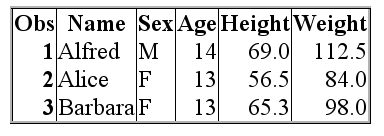
\includegraphics[width=6in]{table_rules.png}
\end{goutput}

\subsection{A Simple Solution}
\index{thead}
\index{Table!thead}
The output looks fine but what is desired is a line between the
Headers and the data.  A little bit of research shows that the
HTML thead tag can have borders.  The thead tag in the output
has no attributes at all.  A border on the bottom
of the tables head section should do the trick.  As confirmation
modifying the thead tag gives the correct look if the
tag looks like this.
\begin{sfvoutput}
<thead style="border-bottom-style: solid;">
\end{sfvoutput}

\subsection{Identify and locate the event}
\index{thead}
\index{Tagsets!HTML4}
\index{Tagsets!HTMLCSS}
\index{Tagsets!PHTML}
\index{Events!table\_head}
Identifying the proper event is easy in this case.
A search for 'thead' in the html tagsets gives us the table\_head event.

It is important to preserve any behavior of the event that is being
redefined.  But in this case there isn't much there.  And the event
is only defined once in the entire htmltags.tpl file.
Looking at the html4 tagset shows no table\_head event.
The parent of html4 is htmlcss, but htmlcss doesn't have a table\_head
event either.  Finally, looking at phtml reveals the table\_head event.
The event is very simple.

\begin{sfvcode}
        define event table_head;
            start:
                put '<thead>' nl;
            finish:
                put '</thead>' nl;
        end;
\end{sfvcode}

\subsection{A Simple Solution}
Changing that will be very simple. The new tagset is shown 
in figure \vref{table_rules1}.
The desired output is shown 
in figure \vref{table_rules1_out}.

\begin{fvcode}{table_rules1}{Columnwise table rules}

proc template;

    define tagset tagsets.table_rules;
        parent=tagsets.html4;

        define event table_head;
            start:
                put '<thead style="border-bottom-style: solid;">' nl;
            finish:
                put '</thead>' nl;
        end;
    end;
run;

ods tagsets.table_rules file='table.html' style=table_rules;
options obs=3;
proc print data=sashelp.class; run;
ods _all_ close;
\end{fvcode}

\begin{goutput}{table_rules1_out}{Columnwise table rules}
\includegraphics[width=6in]{table_rules1.png}
\end{goutput}

\subsection{Table Rules with style}
\index{Events!table\_head}
\index{Styles!table\_head}
Hard coding the style information in the tagset event is certainly
an easy solution.  But there is a better solution.  By using styles
the tagset can be made that will adapt to any need.  All that is really
needed is a style for the table\_head.  Then the tagset needs to use
that style.

Create a new style element for the table\_head is easy.  Setting 
the style on the table\_head
event is also easy.  The only thing that may not be so obvious is that
it is no longer necessary to put a style attribute on the thead tag.
All that is needed is a class attribute that will reference the new
style element.

\subsection{The Better Solution}
The new style and tagset is shown
in figure \ref{table_rules2} on page \pageref{table_rules2}.
The output from this job looks identical to the previous output. The
only difference is the implementation.

\begin{fvcode}{table_rules2}{Table rules with style}

proc template;

    define style styles.table_rules;

        style table /
          borderwidth=3
          bordercolor=black
          rules=cols
        ;

        style table_head /
          borderbottomstyle=solid
        ;
     end;

    define tagset tagsets.table_rules;
        parent=tagsets.html4;

        define event table_head;
            style=table_head;
            start:
                put '<thead'
                putq 'htmlclass=' htmlclass;
                put '>' nl;
            finish:
                put '</thead>' nl;
        end;
    end;
run;

ods tagsets.table_rules file='table.html' style=table_rules;
options obs=3;
proc print data=sashelp.class; run;
ods _all_ close;
\end{fvcode}

This is now a very flexible tagset that will work for anyone.
If no table\_head style is defined then it will behave as always.
But if it is defined, the table head will do whatever is asked 
of it.  

Excercise: Expand on this idea by applying it to the table\_body
and table\_foot events.  Play with the style attributes to see what happens.

\section{Everyone likes stripes}
\index{Table!Striped}
\index{Styles!data}
\index{Styles!dataStrong}
\index{Styles!dataEmphasis}
Another common request is to create tables with striped rows.  This is another
thing that is quite easy to do with styles.  A new style is needed to contrast the
data style already in use.  Then each row should switch between the data style and
the new style.  This is especially easy in SAS 9.1 because of do blocks.

It should be noted, that this can also be done with table templates.  However, 
table templates do not apply to the Report, Tabulate or Print procedures.

\subsection{Defining the Problem}
The goal for this solution is to stripe the data but not the headers or footers.
Reusing existing style elements would be ideal. But creating a new style is not 
out of the question.

\index{Styles!dataStrong}
\index{Styles!dataEmphasis}
\index{Variables!Section}
This is all easy enough to do.  There is a tagset variable called section that
indicates which part of the table the current row is in.  The possible values are head, body,
and foot.  There are also other data style elements available.  Most if not all
styles define dataStrong and dataEmphasis style elements in addition to the data
style.  One of those could be alternated with the data style.  Looking at some of
the style definitions shows that some of them only make the text bold or italic
for these style elements.  That may be too subtle.

For flexibility it would be nice to specify the alternate row style on the ods
statement.  If none is given then the tagset can assume it should use the dataStrong
style.


\subsection{The HTML solution}
\index{Events!classAlign}
\index{HTML!Justification}
\index{HTML!Class}
\index{Tagsets!html4}
\index{Tagsets!htmlcss}
There is no real need to identify and locate these events.  The data, header, row,
and table events figure prominently in most tagsets.
The only real complexity comes when examining the row and data events
in the html4 and htmlcss tagsets.  Instead of just 
printing the htmlclass it triggers an event called classAlign.  This is because
the html output creates a class attribute that has two class names.  One is
for the style and the other is for justification.  Now the classAlign event
needs to be redifined as well. If possible it is best to
preserve the current behavior of any modified events.  In this case the
behavior can be preserved by conditionally limiting the modification to 
only occur when the htmlcass is set to 'data'.

\subsection{The Code}
The finished html tagset is shown below. The striped tabular output is shown 
in figure \ref{striped_table_out} on page \pageref{striped_table_out}.

\begin{fvcode}{striped_table}{The striped table tagset}

proc template;

    define style styles.stripes;
        parent=styles.default;
    
        style DataStripe from data /
            background=cxE0E0E0
        ;
        
    end;
    
    define tagset tagsets.stripes;
        parent=tagsets.html4;

        define event initialize;

            do /if $options;
                 
                set $alt_row_style $options['ROW_STYLE'];
            done;

            set $alt_row_style 'datastrong' /if !$alt_row_style;
        end;

        define event options_set;
            trigger initialize;
        end;

        define event table_head;
            style=table_head;
            start:
                put '<thead';
                putq 'htmlclass=' htmlclass;
                put '>' nl;
                set $row_class 'data';
            finish:
                put '</thead>' nl;
        end;

        define event row;
            start:
                put '<tr>' nl;

            finish:
                put '</tr>' nl;

                do /if cmp(section, 'body');
                    do /if cmp($row_class, 'data');
                        set $row_class $alt_row_style;
                    else;
                        set $row_class 'data';
                    done;
                done;
        end;

        define event classalign;
            do /if cmp(htmlclass, 'data');
                set $class $row_class;
            else;
                set $class htmlclass;
            done;

            unset $vjust;
            unset $just;
            set $vjust vjust / when !cmp("t", vjust);
            set $just just / when !cmp("l", just);
            set $just "r" /when cmp("d", $just);
            break / when !any($class, $just, $vjust);
            put ' class="';
            put $just ' ' $vjust;
            put ' ' $class;
            put '"';
        end;
    end;
run;

ods tagsets.stripes file='striped.html' 
                   options(row_style='datastripe') 
                   style=stripes;
options obs=5;
proc print data=sashelp.class; run;
ods _all_ close;
\end{fvcode}

\begin{goutput}{striped_table_out}{Striped Tables}
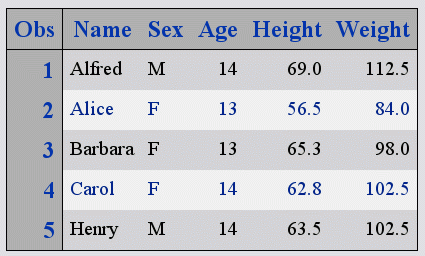
\includegraphics[width=6in]{striped.png}
\end{goutput}

\subsection{The LaTeX solution}
\index{Table!Striped}
\index{LaTeX}
\index{Events!Header}
Doing this same example in LaTeX is even easier.  Mostly because
the LaTeX tagset is not as complicated as the html tagset.
The only difficulty comes from the header event.  The header event
in latex looks like this.
\begin{sfvcode}
        define event header;
            start:
               trigger data;
            finish:
               trigger data;
        end;
\end{sfvcode}

\index{Else}
\index{Statements!Else}
This is fine until the stylename that get's printed is the row\_class
variable.  The result is that all of the header cells are
missing their header references.  The fix was to do this in the data
event.   A Do / else block would be more efficient, but this works
just fine too.
\begin{sfvcode}
        put $row_class /if !cmp(event_name, 'header');
        put htmlclass  /if cmp(event_name, 'header');
\end{sfvcode}

\subsection{The Code}
The finish tagset is shown below. The output is shown 
in figure \vref{striped_table2_out}.

\begin{fvcode}{striped_table2}{Striped tables complete}

proc template;

    define tagset tagsets.striped_latex;
        parent=tagsets.colorlatex;

        define event initialize;

            do /if $options;
                 
                set $alt_row_style $options['ROW_STYLE'];
            done;

            set $alt_row_style 'datastrong' /if !$alt_row_style;
        end;

        define event options_set;
            trigger initialize;
        end;

        define event table_body;
            start:
                set $row_class 'Data';
            finish:
                unset $row_class;
        end;

        define event row;
            finish:
                put CR '\\\hline' CR;

                do /if cmp(section, 'body');
                    do /if cmp($row_class, 'Data');
                        set $row_class $alt_row_style;
                    else;
                        set $row_class 'Data';
                    done;
                done;
        end;

        define event data;
            start:
                put VALUE /if cmp($sascaption, 'true');
                break /if cmp($sascaption, 'true');
                put ' & ' CR / if !cmp(COLSTART, '1') ;

                /* Print cell formatting including class name and alignment. */
                put '   ';
                put '\multicolumn{';
                put colspan;
                put '1' / if !exists(colspan);
                put '}';
                put '{|S{';
                put $row_class /if !cmp(event_name, 'header');
                put htmlclass  /if cmp(event_name, 'header');
                put '}{';
                put just;
                put '}|}';
                put '{';
                put VALUE;

            finish:
                break /if cmp($sascaption, 'true');
                put '}';
        end;
 
    end;
run;

ods tagsets.striped_latex 
    file='striped.tex' 
    style=stripes 
    options(row_style="DataStripe");

options obs=5;
proc print data=sashelp.class; run;
ods _all_ close;
\end{fvcode}


\begin{table}\caption{Striped LaTeX Table}
\label{striped_table2_out}
\begin{sastable}[c]{rllrrr}\hline
   \multicolumn{1}{|S{Header}{c}|}{Obs} & 
   \multicolumn{1}{|S{Header}{c}|}{Name} & 
   \multicolumn{1}{|S{Header}{c}|}{Sex} & 
   \multicolumn{1}{|S{Header}{c}|}{Age} & 
   \multicolumn{1}{|S{Header}{c}|}{Height} & 
   \multicolumn{1}{|S{Header}{c}|}{Weight}
\\\hline
   \multicolumn{1}{|S{RowHeader}{r}|}{ 1} & 
   \multicolumn{1}{|S{Data}{l}|}{Alfred} & 
   \multicolumn{1}{|S{Data}{l}|}{M} & 
   \multicolumn{1}{|S{Data}{r}|}{14} & 
   \multicolumn{1}{|S{Data}{r}|}{69.0} & 
   \multicolumn{1}{|S{Data}{r}|}{112.5}
\\\hline
   \multicolumn{1}{|S{RowHeader}{r}|}{ 2} & 
   \multicolumn{1}{|S{DataStripe}{l}|}{Alice} & 
   \multicolumn{1}{|S{DataStripe}{l}|}{F} & 
   \multicolumn{1}{|S{DataStripe}{r}|}{13} & 
   \multicolumn{1}{|S{DataStripe}{r}|}{56.5} & 
   \multicolumn{1}{|S{DataStripe}{r}|}{ 84.0}
\\\hline
   \multicolumn{1}{|S{RowHeader}{r}|}{ 3} & 
   \multicolumn{1}{|S{Data}{l}|}{Barbara} & 
   \multicolumn{1}{|S{Data}{l}|}{F} & 
   \multicolumn{1}{|S{Data}{r}|}{13} & 
   \multicolumn{1}{|S{Data}{r}|}{65.3} & 
   \multicolumn{1}{|S{Data}{r}|}{ 98.0}
\\\hline
   \multicolumn{1}{|S{RowHeader}{r}|}{ 4} & 
   \multicolumn{1}{|S{DataStripe}{l}|}{Carol} & 
   \multicolumn{1}{|S{DataStripe}{l}|}{F} & 
   \multicolumn{1}{|S{DataStripe}{r}|}{14} & 
   \multicolumn{1}{|S{DataStripe}{r}|}{62.8} & 
   \multicolumn{1}{|S{DataStripe}{r}|}{102.5}
\\\hline
   \multicolumn{1}{|S{RowHeader}{r}|}{ 5} & 
   \multicolumn{1}{|S{Data}{l}|}{Henry} & 
   \multicolumn{1}{|S{Data}{l}|}{M} & 
   \multicolumn{1}{|S{Data}{r}|}{14} & 
   \multicolumn{1}{|S{Data}{r}|}{63.5} & 
   \multicolumn{1}{|S{Data}{r}|}{102.5}
\\\hline
\end{sastable}
\end{table}

\subsection{Summary}
With just a little extra effort the striped tagsets provide enough
flexibility to be useful with any style.  They can even provide
different looks by using different style elements within the chosen
style.  If the style doesn't provide a suitable style element then
it is still easy to inherit from that style and add a single element
to do the striping.

Excercise:  It would be a worthwhile to play with different
styles and style elements to see what sort of striping you might
get.

\section{slidebar columns}
This is a great example of what can be done with a little
imagination.  This example takes advantage of cell widths
as percentages, to create a bar chart affect within a table column.

\subsection{Define the Problem}
The desire is to use a numeric or percentage value and 
create a sliding bar that reflects the value.  If it's a percentage
everything is very easy.  If it is a numeric value then things get
a little more complicated.  Those cases will need some sort of maximum
value to create a percentage from.  Another need is how to
identify the column to use.  For this, styles will be used in a new way.

The HTML implementation of the slidebar is done by creating a table 
inside the data cell.  The table will have 2 cells inside of it.  
The first one will use a percentage width to create a bar.  A little bit of
HTML editing shows that a table cell like this one will give the
desired effect.

\begin{sfvcode}
    <td width="150">
      <table width="100%">
        <td width="72%">72</td><td>&nbsp;</td>
      </table>
    </td>
\end{sfvcode}

\index{Style!Attributes!TagAttr}
\index{Style!Attributes!HTMLClass}
\label{slider}
There is a style attribute called TagAttr.  It stands for Tag Attribute.
TagAttr was meant as a catch all
for any new browser features that styles did not directly accomodate.
Normally anything in TagAttr is printed as is within the tag it belongs
to.  This tagset is going to misuse TagAttr so that proc print can say which columns
should get a slide bar.  It can also be used to give the maximum value for
columns that are not percentages.

\subsection{Identify and Locate}
This step get's easier as tagset events become familiar.  
In this case everything revolves around the data event. 

\subsection{The Solution}
Let's get on with the code. 

\begin{fvcode}{final_slider}{Slider Tagset Complete}
proc template;
    define style styles.slider;
        parent=styles.default;

        style table from output /
            rules=cols
            cellpadding=3
            cellspacing=1
        ;
        style slider from data /
            background=colors('headerbg')
        ;
    end;
  
    define tagset tagsets.slider;
        parent=tagsets.html4;

        define event calculate_width;
            set $width value /breakif index(value, '%') > 0;

            eval $dash_pos index(Tagattr, '-');
            do /if $dash_pos;
                eval $dash_pos $dash_pos+1;
            done;
            eval $value inputn(value, '12.');
            eval $max inputn(substr(Tagattr, $dash_pos), '12.');
            eval $width ($value / $max) * 100;
            set $width $width '%';
            unset $dash_pos;
        end;

        define event data;
            start:
                /* this would work but sometimes htmlclass is empty... */
                trigger header /breakif cmp(htmlclass, "RowHeader");
                trigger header /breakif cmp(htmlclass, "Header");

                do /if index(tagattr, 'slider') > 0;
                    put '<td width="150" class="data">' nl;
                    put '<table width="100%" class="data" cellpadding=0; cellspacing=0;>' nl;
                    trigger calculate_width;
                done;
                put "<td";
                putq ' width=' $width;
                putq " title=" flyover;
                do /if !cmp(htmlclass,'batch');
                    trigger classalign;
                    trigger style_inline;
                done;
                trigger rowcol;
                put " nowrap" /if no_wrap;
                put ">";
                trigger cell_value;

            finish:
                trigger header /breakif cmp(htmlclass, "RowHeader");
                trigger header /breakif cmp(htmlclass, "Header");
   
                trigger cell_value;
                put "</td>" CR;
                do /if $width;
                    put '<td>&nbsp;</td>' CR;
                    put "</table></td>" CR;
                    unset $width;
                done;

        end;
    end;
run;

options obs=3;
ods tagsets.slider file='test.html' style=slider;

proc print data=sashelp.class;
    var name;
    var sex;
    var age;     
    var height / style(data) = slider[just=center tagattr="slider-80"];
    var weight / style(data) = slider[just=center tagattr="slider-150"];
run;

ods tagsets.slider close;
\end{fvcode}        

The output from this example can be seen in figure \vref{slider_out}.
The heart of this example is the data event.  
All it needed was an if block that would create a table with two
cells inside what would ordinarily be a simple data cell.  The first cell
in the slider table is created with the code that normally creates the data
cell.  It just adds the \$width variable if it is there.  The finish
of the data event adds the extra empty cell and closes everything up.

The most complicated part of the tagset is the calculate\_width event.
This is mostly because sliders will work for numeric values as well as
percentages.
If the tagset only worked with pecentages this event wouldn't have been needed.

There is also a short style to make the table look a little nicer.  
Using less cellspacing and padding along with column rules looks nice.  
This example could be combined with the first example in this chapter
for an even nicer look.

The last piece of the puzzle is using the print Procedure's style over-ride
capabilities to turn the sliders on and give a max value to calculate
the percentages from.  A macro variable could have been used to
indicate which columns to use, but this is a little bit nicer.

Excercise:  Create a slider tagset that uses a macro variable or style
over-ride to create sliders on the the columns indicated.

\begin{goutput}{Slider_out}{Slider Columns}
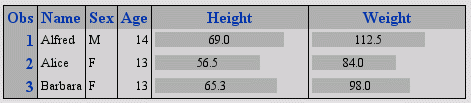
\includegraphics[width=6in]{slider.png}
\end{goutput}

\subsection{Example Summary}
In this example the tagattr style attribute was used to indicate the 
slider columns and the
maximum value.  But since a slider style element was also created the
tagset could just as easily key off of the value of htmlclass and only 
use tagattr to indicate a maximum value if needed.

Exercise: Find and eliminate the extra printing of Tagattr in the data tags.

Exercise: Change the tagset to key off of the style element name instead of
the keyword 'slider' in tagattr.

Exercise: Change the inheritance of this tagset to take advantage of the
changes made to the table\_rules tagset in figure \ref{table_rules2} on page
\pageref{table_rules2}. Combine the table\_rules style with
the slider style.

Exercise: Combine all the examples in the chapter into one tagset.

\section{Summary}
This chapter has shown how styles can be used with tagsets to easily create
nice output.  Using styles can simplify solutions and make those solutions
more adaptable. 
